\documentclass{standalone}
\usepackage{tikz}
\usetikzlibrary{automata, positioning, arrows}

\begin{document}

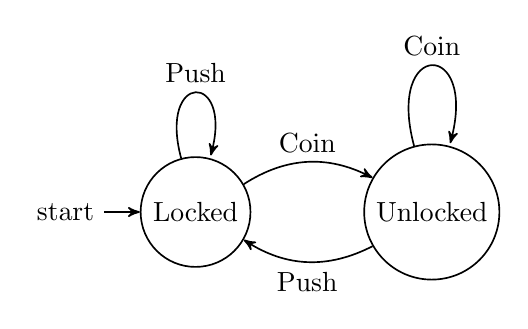
\begin{tikzpicture}[->, >=stealth', auto, semithick, node distance=3cm]
\tikzstyle{every state}=[fill=white,draw=black,text=black]

\node[state, initial] (L) {Locked};
\node[state] (U) [right of=L] {Unlocked};

\path
(L) edge[bend left]  node{Coin} (U)
(U) edge[bend left]  node{Push} (L)
(L) edge[loop above] node{Push} (L)
(U) edge[loop above] node{Coin} (U);

\end{tikzpicture}

\end{document}
